% \newcommand{\compacttitlespacing}{0} %disable when we need room for authors
\documentclass[sigconf]{acmart}
\settopmatter{printacmref=false}
% defining the \BibTeX command - from Oren Patashnik's original BibTeX documentation.
\def\BibTeX{{\rm B\kern-.05em{\sc i\kern-.025em b}\kern-.08emT\kern-.1667em\lower.7ex\hbox{E}\kern-.125emX}}
    
\usepackage{nicefrac}
\usepackage{siunitx}
\usepackage{array,framed}
\usepackage{booktabs}
\usepackage{
  color,
  float,
  epsfig,
  wrapfig,
  graphics,
  graphicx,
  subcaption
}
% \usepackage[dvipsnames]{xcolor}
\usepackage{textcomp,amssymb}
\usepackage{setspace}
% \usepackage{amsfonts}
\usepackage{latexsym,fancyhdr,url}
\usepackage{enumerate}
\usepackage{algorithm2e}
\usepackage{algpseudocode}
\usepackage{graphics}
\usepackage{xparse} % argument parsing -- \edist
\usepackage{xspace}
\usepackage{multirow}
\usepackage{csvsimple}
\usepackage{balance}
\usepackage{csquotes}
% \usepackage{flushend}
% \usepackage{mathptmx,avant}

%%%% Tikz variables, pgfplot
\usepackage{
  tikz,
  pgfplots,
  pgfplotstable
}
\usepackage{hyperref}
\hypersetup{
    colorlinks=true,
    linkcolor=black,
    % filecolor=magenta,      
    urlcolor=blue,
    citecolor =black,
}
\usepackage{listings}
\usepackage{xcolor}

    \definecolor{codegreen}{rgb}{0,0.6,0}
    \definecolor{codegray}{rgb}{0.5,0.5,0.5}
    \definecolor{codepurple}{rgb}{0.58,0,0.82}
    \definecolor{backcolour}{rgb}{0.95,0.95,0.92}
    
\lstdefinestyle{paulito}{
    backgroundcolor=\color{backcolour},   
    commentstyle=\color{codegreen},
    keywordstyle=\color{magenta},
    numberstyle=\tiny\color{codegray},
    stringstyle=\color{codepurple},
    basicstyle=\ttfamily\footnotesize,
    breakatwhitespace=false,         
    breaklines=true,                 
    captionpos=b,                    
    keepspaces=true,                 
    numbers=left,                    
    numbersep=5pt,                  
    showspaces=false,                
    showstringspaces=false,
    showtabs=false,                  
    tabsize=2
}
\lstset{style=paulito}


\usetikzlibrary{
  shapes.geometric,
  arrows,
  external,
  pgfplots.groupplots,
  matrix
}

\pgfplotsset{compat=1.9}
% \tikzexternalize[prefix=images/]
% \tikzexternalenable

%\pagenumbering{arabic}
% \pagestyle{plain}

\usepackage{mathtools,}
\DeclarePairedDelimiter\abs{\lvert}{\rvert}
\DeclarePairedDelimiter\norm{\lVert}{\rVert}

% \setmathfont{Latin Modern Math}[version=lm]
\DeclareMathAlphabet{\mathcal}{OMS}{cmsy}{m}{n}
% \DeclareSymbolFont{operators}{T1}{cmr}{m}{n}
% \DeclareSymbolFont{letters}{OML}{cmm}{m}{it}
% \DeclareSymbolFont{symbols}{OMS}{cmsy}{m}{n}
% \DeclareSymbolFont{largesymbols}{OMX}{cmex}{m}{n}

% \usepackage{times}

% \setmathcal{Arial}

% TO deal with the weird flow of boxes
% \brokenpenalty=1000
% \clubpenalty=1000
% \widowpenalty=10
\DeclareGraphicsExtensions{%
    .png,.PNG,%
    .pdf,.PDF,%
    .jpg,.mps,.jpeg,.jbig2,.jb2,.JPG,.JPEG,.JBIG2,.JB2}

\usepackage{xparse}
\newcommand{\bnm}{\begin{newmath}}
\newcommand{\enm}{\end{newmath}}

\newcommand{\bea}{\begin{eqnarray*}}%
\newcommand{\eea}{\end{eqnarray*}}%

\newcommand{\bne}{\begin{newequation}}
\newcommand{\ene}{\end{newequation}}

\newcommand{\bal}{\begin{newalign}}
\newcommand{\eal}{\end{newalign}}

\newenvironment{newalign}{\begin{align}%
\setlength{\abovedisplayskip}{4pt}%
\setlength{\belowdisplayskip}{4pt}%
\setlength{\abovedisplayshortskip}{6pt}%
\setlength{\belowdisplayshortskip}{6pt} }{\end{align}}

\newenvironment{newmath}{\begin{displaymath}%
\setlength{\abovedisplayskip}{4pt}%
\setlength{\belowdisplayskip}{4pt}%
\setlength{\abovedisplayshortskip}{6pt}%
\setlength{\belowdisplayshortskip}{6pt} }{\end{displaymath}}

\newenvironment{neweqnarrays}{\begin{eqnarray*}%
\setlength{\abovedisplayskip}{-4pt}%
\setlength{\belowdisplayskip}{-4pt}%
\setlength{\abovedisplayshortskip}{-4pt}%
\setlength{\belowdisplayshortskip}{-4pt}%
\setlength{\jot}{-0.4in} }{\end{eqnarray*}}

\newenvironment{newequation}{\begin{equation}%
\setlength{\abovedisplayskip}{4pt}%
\setlength{\belowdisplayskip}{4pt}%
\setlength{\abovedisplayshortskip}{6pt}%
\setlength{\belowdisplayshortskip}{6pt} }{\end{equation}}


\newcounter{ctr}
\newcounter{savectr}
\newcounter{ectr}

\newenvironment{newitemize}{%
\begin{list}{\mbox{}\hspace{5pt}$\bullet$\hfill}{\labelwidth=15pt%
\labelsep=4pt \leftmargin=12pt \topsep=3pt%
\setlength{\listparindent}{\saveparindent}%
\setlength{\parsep}{\saveparskip}%
\setlength{\itemsep}{3pt} }}{\end{list}}


\newenvironment{newenum}{%
\begin{list}{{\rm (\arabic{ctr})}\hfill}{\usecounter{ctr} \labelwidth=17pt%
\labelsep=5pt \leftmargin=22pt \topsep=3pt%
\setlength{\listparindent}{\saveparindent}%
\setlength{\parsep}{\saveparskip}%
\setlength{\itemsep}{2pt} }}{\end{list}}

%%%%%%%%%%%%%%%%%%%%%%%%%%%%%%%%%%%%%%%%%%%%%%%%%%%%%%%%%%%%%%%%%%%%%%%%%%%%%%
%
% Figure and table macros
%

\newcounter{mytable}
\def\mytable{\begin{centering}\refstepcounter{mytable}}
\def\endmytable{\end{centering}}

\def\mytablecaption#1{\vspace{2mm}
  \centerline{Table \arabic{mytable}.~{#1}}
  \vspace{6mm}
  \addcontentsline{lot}{table}{\protect\numberline{\arabic{mytable}}~{#1}}
}


\newcounter{myfig}
\def\myfig{\begin{centering}\refstepcounter{myfig}}
\def\endmyfig{\end{centering}}

\def\myfigcaption#1{
             \vspace{2mm}
             \centerline{\textsf{Figure \arabic{myfig}.~{#1}}}
             \vspace{6mm}
             \addcontentsline{lof}{figure}{\protect\numberline{\arabic{myfig}}~{#1}}}


\newlength{\saveparindent}
\setlength{\saveparindent}{\parindent}
\newlength{\saveparskip}
\setlength{\saveparskip}{\parskip}

\newcommand{\decOracle}{\textbf{Dec}}

\newcommand{\negsmidge}{{\hspace{-0.1ex}}}
\newcommand{\cdotsm}{\negsmidge\negsmidge\negsmidge\cdot\negsmidge\negsmidge\negsmidge}

\def\suchthatt{\: :\:}
\newcommand{\E}{{\rm I\kern-.3em E}}
\newcommand{\Prob}[1]{{\Pr\left[\,{#1}\,\right]}}
\newcommand{\Probb}[2]{{\Pr}_{#1}\left[\,{#2}\,\right]}
\newcommand{\CondProb}[2]{{\Pr}\left[\: #1\:\left|\right.\:#2\:\right]}
\newcommand{\CondProbb}[2]{\Pr[#1|#2]}
\newcommand{\ProbExp}[2]{{\Pr}\left[\: #1\:\suchthatt\:#2\:\right]}
\newcommand{\Ex}[1]{{\textnormal{E}\left[\,{#1}\,\right]}}
\newcommand{\Exx}{{\textnormal{E}}}
\newcommand{\given}{\ensuremath{\,\big|\,}}


\newcommand{\true}{\mathsf{true}}
\newcommand{\false}{\mathsf{false}}
\def\negl{\mathsf{negl}}


\newcommand{\secref}[1]{\mbox{Section~\ref{#1}}}
\newcommand{\appref}[1]{\mbox{Appendix~\ref{#1}}}
\newcommand{\thref}[1]{\mbox{Theorem~\ref{#1}}}
\newcommand{\defref}[1]{\mbox{Definition~\ref{#1}}}
\newcommand{\corref}[1]{\mbox{Corollary~\ref{#1}}}
\newcommand{\lemref}[1]{\mbox{Lemma~\ref{#1}}}
\newcommand{\clref}[1]{\mbox{Claim~\ref{#1}}}
\newcommand{\propref}[1]{\mbox{Proposition~\ref{#1}}}
\newcommand{\factref}[1]{\mbox{Fact~\ref{#1}}}
\newcommand{\remref}[1]{\mbox{Remark~\ref{#1}}}
\newcommand{\figref}[1]{\mbox{Figure~\ref{#1}}}
\renewcommand{\algref}[1]{\mbox{Algorithm~\ref{#1}}}
% \newcommand{\eqref}[1]{\mbox{Equation~(\ref{#1})}}
% Have to use \renewcommand because exists already in amsmath
\renewcommand{\eqref}[1]{\mbox{Equation~(\ref{#1})}}
\newcommand{\consref}[1]{\mbox{Construction~\ref{#1}}}
\newcommand{\tabref}[1]{\mbox{Table~\ref{#1}}}

\newcommand{\get}{{\:{\leftarrow}\:}}
\newcommand{\gett}[1]{\:{\leftarrow}_{#1}\:}
\newcommand{\getsr}{{\:{\leftarrow{\hspace*{-3pt}\raisebox{.75pt}{$\scriptscriptstyle\$$}}}\:}}
\newcommand{\getm}{{\:\leftarrow_{\mdist}\:}}
\newcommand{\getd}{{\:\leftarrow_{\ddist}\:}}
%\newcommand{\getm}{{\:{\leftarrow{\hspace*{-3pt}\raisebox{.75pt}{$\scriptscriptstyle \mdist$}}}\:}}
\newcommand{\getk}{{\:\leftarrow_{\kdist}\:}}
%\newcommand{\getk}{{\:{\leftarrow{\hspace*{-3pt}\raisebox{.75pt}{$\scriptscriptstyle \kdist$}}}\:}}
\newcommand{\getp}{{\:\leftarrow_{p}\:}}



\newcommand{\gamesfontsize}{\small}
\newcommand{\fpage}[2]{\framebox{\begin{minipage}[t]{#1\textwidth}\setstretch{1.1}\gamesfontsize  #2 \end{minipage}}}
\newcommand{\mpage}[2]{\begin{minipage}[t]{#1\textwidth}\setstretch{1.1}\gamesfontsize  #2 \end{minipage}}

\newcommand{\hpages}[3]{\begin{tabular}{cc}\begin{minipage}[t]{#1\textwidth} #2 \end{minipage} & \begin{minipage}[t]{#1\textwidth} #3 \end{minipage}\end{tabular}}

\newcommand{\hpagess}[4]{
        \begin{tabular}[t]{c@{\hspace*{.5em}}c}
        \begin{minipage}[t]{#1\textwidth}\gamesfontsize #3 \end{minipage}
        &
        \begin{minipage}[t]{#2\textwidth}\gamesfontsize #4 \end{minipage}
        \end{tabular}
    }

\newcommand{\hpagesss}[6]{
        \begin{tabular}[t]{c@{\hspace*{.5em}}c@{\hspace*{.5em}}c@{\hspace*{.5em}}c}
        \begin{minipage}[t]{#1\textwidth}\gamesfontsize #4 \end{minipage}
        &
        \begin{minipage}[t]{#2\textwidth}\gamesfontsize #5 \end{minipage}
        &
        \begin{minipage}[t]{#3\textwidth}\gamesfontsize #6 \end{minipage}
        \end{tabular}
    }

\newcommand{\hpagessss}[8]{
        \begin{tabular}{c@{\hspace*{.5em}}c@{\hspace*{.5em}}c@{\hspace*{.5em}}c}
        \begin{minipage}[t]{#1\textwidth}\gamesfontsize #5 \end{minipage}
        &
        \begin{minipage}[t]{#2\textwidth}\gamesfontsize #6 \end{minipage}
        &
        \begin{minipage}[t]{#3\textwidth}\gamesfontsize #7 \end{minipage}
        &
        \begin{minipage}[t]{#4\textwidth}\gamesfontsize #8 \end{minipage}
        \end{tabular}
    }


\newcommand{\hfpages}[3]{\hfpagess{#1}{#1}{#2}{#3}}
\newcommand{\hfpagess}[4]{
        \begin{tabular}[t]{c@{\hspace*{.5em}}c}
        \framebox{\begin{minipage}[t]{#1\textwidth}\setstretch{1.1}\gamesfontsize #3 \end{minipage}}
        &
        \framebox{\begin{minipage}[t]{#2\textwidth}\setstretch{1.1}\gamesfontsize #4 \end{minipage}}
        \end{tabular}
    }
\newcommand{\hfpagesss}[6]{
        \begin{tabular}[t]{c@{\hspace*{.5em}}c@{\hspace*{.5em}}c}
        \framebox{\begin{minipage}[t]{#1\textwidth}\setstretch{1.1}\gamesfontsize #4 \end{minipage}}
        &
        \framebox{\begin{minipage}[t]{#2\textwidth}\setstretch{1.1}\gamesfontsize #5 \end{minipage}}
        &
        \framebox{\begin{minipage}[t]{#3\textwidth}\setstretch{1.1}\gamesfontsize #6 \end{minipage}}
        \end{tabular}
    }
\newcommand{\hfpagessss}[8]{
        \begin{tabular}[t]{c@{\hspace*{.5em}}c@{\hspace*{.5em}}c@{\hspace*{.5em}}c}
        \framebox{\begin{minipage}[t]{#1\textwidth}\setstretch{1.1}\gamesfontsize #5 \end{minipage}}
        &
        \framebox{\begin{minipage}[t]{#2\textwidth}\setstretch{1.1}\gamesfontsize #6 \end{minipage}}
        &
        \framebox{\begin{minipage}[t]{#3\textwidth}\setstretch{1.1}\gamesfontsize #7 \end{minipage}}
        &
        \framebox{\begin{minipage}[t]{#4\textwidth}\setstretch{1.1}\gamesfontsize #8 \end{minipage}}
        \end{tabular}
    }

\newcommand{\vecw}{\mathbf{w}}
\newcommand{\R}{\mathbb{R}}
\newcommand{\N}{\mathbb{N}}
\newcommand{\Z}{\mathbb{Z}}
\newcommand{\load}{L}
\newcommand{\coll}{\mathsf{Coll}}
\newcommand{\nocoll}{\overline{\mathsf{Coll}}}


\newcommand{\Img}{\textsf{Img}}

%%%%%%%%%%%%%%%%%%%%%%%%%%%%%%%%%%%%%%%%%%%%%%%%%%%%%%%%%%%%%%%%%%%%%%%%%%%%%%%%
%%%% Fonts and symbols
%%%%%%%%%%%%%%%%%%%%%%%%%%%%%%%%%%%%%%%%%%%%%%%%%%%%%%%%%%%%%%%%%%%%%%%%%%%%%%%%
\newcommand\funcfont{\textsf}
\newcommand\variablefont{\texttt}

%%%%%%%%%%%%%%%%%%%%%%%%%%%%%%%%%%%%%%%%%%%%%%%%%%%%%%%%%%%%%%%%%%%%%%%%%%%%%%%%
%%%%%%%%%%%%%%%%%%%%%%%%%%%%%%%% NEW COMMANDS %%%%%%%%%%%%%%%%%%%%%%%%%%%%%%%%%%
%%%%%%%%%%%%%%%%%%%%%%%%%%%%%%%%%%%%%%%%%%%%%%%%%%%%%%%%%%%%%%%%%%%%%%%%%%%%%%%%

\def \Perm {\funcfont{Perm}}
\def \calC {{\mathcal{C}}}
\def \calU {{\mathcal{U}}}
\renewcommand{\u}{\ensuremath{u}}
\newcommand{\unew}{\ensuremath{\tilde{u}}}

\newcommand{\calN}{\mathcal{N}}
\def \sspace {{\mathcal{S}}}
\def \strings {{\mathcal{S}}}
\def \slen {{s}}
\def \kspace {{\mathcal{K}}}
\def \kspacesize {{m}}
\def \mspacesize {{n}}
\def \kdict {D}
\def \dictsize {d}
\newcommand{\kdist}{p_k}
\newcommand{\mdist}{\ensuremath{{W}}}
\newcommand{\alldist}{\rho}
\newcommand{\pwdist}{\transgen}
\newcommand{\ddist}{\rho_{dec}}
\newcommand{\PWset}{{\mathcal{P}}}  % TODO: fix, same as \pwdist
\newcommand{\PWsetvec}{\vec{\mathcal{P}}}
\newcommand{\PWvec}{\vec{P}}
\newcommand{\domvec}{\vec{D}}
\newcommand{\humanornot}{\vec{h}}
\newcommand{\dom}{\textsf{dom}}
%\def \kdist {{\kappa}}
%\def \mdist {{\mu}}
%\def \ddist {{\delta}}
\def \pspace {{\mathcal{P}}}
\def \mpspace {{\mathcal{MP}}}
\def \cspace {{\mathcal{C}}}
\def \key {\kappa}
\def \msg {M}
\def \seed {S}
\def \ctxt {C}
\def \ctxtpart {C_2}
\newcommand{\genprime}{{\textsf{GenPrime}}}
\newcommand{\isprime}{{\textsf{IsPrime}}}
\newcommand{\LeastLesserPrime}{{\textsf{PrevPrime}}}
\newcommand{\pwset}{\mathcal{S}}
\newcommand{\DTE}{{\textsf{DTE}}}
\newcommand{\encode}{{\textsf{encode}}}
\newcommand{\decode}{{\textsf{decode}}}

\newcommand{\DTEsingle}{{\textsf{1PW-DTE}}}
\newcommand{\encodesingle}{{\textsf{1PW-encode}}}
\newcommand{\decodesingle}{{\textsf{1PW-decode}}}

\newcommand{\DTErss}{{\textsf{RSS-DTE}}}
\newcommand{\encoderss}{{\textsf{RSS-encode}}}
\newcommand{\decoderss}{{\textsf{RSS-decode}}}

\newcommand{\DTEindep}{{\textsf{MPW-DTE}}}
\newcommand{\encodeindep}{{\textsf{MPW-encode}}}
\newcommand{\decodeindep}{{\textsf{MPW-decode}}}


\newcommand{\DTEsub}{{\textsf{SG-DTE}}}
\newcommand{\encodesub}{{\textsf{SG-encode}}}
\newcommand{\decodesub}{{\textsf{SG-decode}}}
\newcommand{\decodekamf}{{\textsf{KAMF-decode}}}
\newcommand{\DTEis}{{\textsf{IS-DTE}}}
\newcommand{\encodeis}{{\textsf{is-encode}}}
\newcommand{\decodeis}{{\textsf{is-decode}}}
\newcommand{\DTErej}{{\textsf{REJ-DTE}}}
\newcommand{\encoderej}{{\textsf{rej-encode}}}
\newcommand{\decoderej}{{\textsf{rej-decode}}}
\newcommand{\DTErsarej}{{\textsf{RSA-REJ-DTE}}}
\newcommand{\encodeRSAREJ}{{\textsf{rsa-rej-encode}}}
\newcommand{\decodeRSAREJ}{{\textsf{rsa-rej-decode}}}
\newcommand{\DTErsainc}{{\textsf{RSA-INC-DTE}}}
\newcommand{\encodeRSAINC}{{\textsf{rsa-inc-encode}}}
\newcommand{\decodeRSAINC}{{\textsf{rsa-inc-decode}}}
\newcommand{\DTEunf}{{\textsf{UNF-DTE}}}
\newcommand{\DTEnunf}{{\textsf{NUNF-DTE}}}


%\newcommand{\encodeis}{{\textsf{encode}_{\textrm{is}}}}
%\newcommand{\decodeis}{{\textsf{decode}_{\textrm{is}}}}
\newcommand{\rep}{\textsf{rep}}
\newcommand{\isErr}{\epsilon_{\textnormal{is}}}
\newcommand{\incErr}{\epsilon_{\textnormal{inc}}}
\def \enc {{\textsf{E}}}
\def \dec {{\textsf{D}}}
\def \SEscheme {{\textsf{SE}}}
\def \HEscheme {{\textsf{HE}}}
\def \CTR {{\textsf{CTR}}}
\def \encHE {{\textsf{HEnc}}}
\def \HIDE {{\textsf{HiaL}}}
\def \encHIDE {{\textsf{HEnc}}}
\def \decHIDE {{\textsf{HDec}}}
\def \decHE {{\textsf{HDec}}}
\def \encHEt {{\textsf{HEnc2}}}
\def \decHEt {{\textsf{HDec2}}}

\newcommand{\myind}{\hspace*{1em}}
\newcommand{\thh}{^{\textit{th}}} % th
\newcommand{\concat}{\,\|\,}
\newcommand{\dotdot}{..}
\newcommand{\emptystr}{\varepsilon}

\newcommand{\round}{\textsf{round}}

\newcommand{\alphabar}{\overline{\alpha}}
\newcommand{\numbinsbar}{\overline{b}}
\newcommand{\numballs}{a}
\newcommand{\numbins}{b}

%\def \encHE {{\sf{enc}^{HE}}}
%\def \decHE {{\sf{dec}^{HE}}}
%\def \encHEt {{\sf{enc}^{HE2}}}
%\def \decHEt {{\sf{dec}^{HE2}}}
\def \idealHE {{\mathcal{HE}}}
\def \IEnc {{\mathbf{\rho}}}
\def \IDec {{\mathbf{\rho^{-1}}}}
\def \OEnc {{\mathbf{Enc}}}
\def \ODec {{\mathbf{Dec}}}
\newcommand{\SimuProc}{\mathbf{Sim}}
\newcommand{\ROProc}{\mathbf{RO}}
\newcommand{\PrimProc}{\mathbf{Prim}}
\def \stm {g}
\def \istm {\hat{g}}
\def \kts {{f}}
\def \lex {{\sf lex}}
\def \part {part}
\def \kd {{\sf{kd}}}
\def \msgdist {{d}}
\def \keydist {{r}}
\def \ind {{\sf{index}}}
\def \kprf {z}
\def \adv {{\mathcal A}}
\def \pwds {u}
\newcommand{\mpw}{mpw}
\newcommand{\pw}{w}
\newcommand{\pwvec}{\vec{\pw}}
\newcommand{\vecx}{\vec{x}}
\def \tokens {v}
\def \calP{{\mathcal{P}}}
\def \template{{\mathcal{T}}}
\def \vaultset{{\mathcal{V}}}
\def \ext {{\sf ext}}
\def \offset {\delta}
\def \maxweight {\epsilon}
\def \advo {{\mathcal{A}}^{*}}

\newcommand{\Chall}{\textsf{Ch}}
\newcommand{\Test}{\textnormal{\textsf{Test}}}
\newcommand{\RoR}{\textsf{RoR}}
\newcommand{\MI}{\textnormal{MI}}
\providecommand{\MR}{\textnormal{MR}}
\newcommand{\MRCCA}{\textnormal{MR-CCA}}
\newcommand{\SAMP}{\textnormal{SAMP}}
\newcommand{\DTEgame}{\textnormal{SAMP}}
\newcommand{\KR}{\textnormal{KR}}
\newcommand{\advA}{{\mathcal{A}}}
\newcommand{\advR}{{\mathcal{R}}}
\newcommand{\advB}{{\mathcal{B}}} % 
\newcommand{\advC}{{\mathcal{C}}} % C
\newcommand{\advD}{{\mathcal{D}}} % D
\newcommand{\advE}{{\mathcal{E}}}
\newcommand{\advF}{{\mathcal{F}}}
\newcommand{\advG}{{\mathcal{G}}}
\newcommand{\advI}{{\mathcal{I}}}
\newcommand{\nextval}{\;;\;}
\newcommand{\TabC}{\texttt{C}}
\newcommand{\TabR}{\texttt{R}}
\newcommand{\Hash}{H}
\newcommand{\Cipher}{\pi}
\newcommand{\CipherInv}{\pi^{-1}}
\newcommand{\simu}{{\mathcal S}}
\newcommand{\prim}{P}
\newcommand{\maxguess}{\gamma}


\newcommand{\bigO}{\mathcal{O}}
\newcommand{\calG}{{\mathcal{G}}}

\def\sqed{{\hspace{5pt}\rule[-1pt]{3pt}{9pt}}}
\def\qedsym{\hspace{2pt}\rule[-1pt]{3pt}{9pt}}

\newcommand{\Colon}{{\::\;}}
\newcommand{\good}{\textsf{Good}}

\newcommand\Tvsp{\rule{0pt}{2.6ex}}
\newcommand\Bvsp{\rule[-1.2ex]{0pt}{0pt}}
\newcommand{\TabPad}{\hspace*{5pt}}
\newcommand\TabSep{@{\hspace{5pt}}|@{\hspace{5pt}}}
\newcommand\TabSepLeft{|@{\hspace{5pt}}}
\newcommand\TabSepRight{@{\hspace{5pt}}|}


\DeclareMathOperator*{\argmin}{argmin}
\DeclareMathOperator*{\argmax}{argmax}
\newcommand{\comma}{\textnormal{,}}

\renewcommand{\paragraph}[1]{\vspace*{6pt}\noindent\textbf{#1}\;}

\newcommand{\weirvault}{\textsf{Pastebin}\xspace}
\newcommand{\ndssvault}{\textsf{DBCBW}\xspace}




\newcommand{\reminder}[1]{ [[[ \marginpar{\mbox{$<==$}} #1 ]]] }

%
% New theorem types: (Already in CCS template)
%
\newtheorem{observation}{Observation}
%\newtheorem{definition}{Definition}
\newtheorem{claim}{Claim}
\newtheorem{assumption}{Assumption}
\newtheorem{fact}{Fact}
% \newtheorem{theorem}{Theorem}[section]
% \newtheorem{lemma}{Lemma}[section]
% \newtheorem{corollary}{Corollary}[section]
% \newtheorem{proposition}{Proposition}
% \newtheorem{example}{Example}

%
% Definitions:
%
\def \blackslug{\hbox{\hskip 1pt \vrule width 4pt height 8pt
    depth 1.5pt \hskip 1pt}}
\def \qed{\quad\blackslug\lower 8.5pt\null\par}
% In-line QED, for ending a proof with a $$ formula
% In-line QED, for ending a proof with a $$ formula
\def \inQED{\quad\quad\blackslug}
\def \Qed{\QED}
\def \QUAD{$\Box$}
\def \Proof{\par\noindent{\bf Proof:~}}
\def \proof{\Proof}
\def \poly {\mbox{$\mathsf{poly}$}}
\def \binary {\mbox{$\mathsf{binary}$}}
\def \ones {\mbox{$\mathsf{ones}$}}
\def \rank {\mbox{$\mathsf{rank}$}}
\def \bits {\mbox{$\mathsf{bits}$}}
\def \factorial {\mbox{$\mathsf{factorial}$}}
\def \fr {\mbox{$\mathsf{fr}$}}
\def \pr {\mbox{$\mathsf{pr}$}}
\def \zon {\{0,1\}^n}
\def \zo  {\{0,1\}}
\def \zok {\{0,1\}^k}
\def \mo {s}


\def\utilcnt{\ensuremath{\mu_{\mathrm{cnt}}}}
\def\utiltime{\ensuremath{\mu_{\mathrm{time}}}}
\def\ex{\ensuremath{{\mathrm{ex}}}}
\def\rlx{\ensuremath{{\mathrm{rlx}}}}
\def\tp{\textsf{TP}}
\def\cp{\textnormal{\textsf{CP}}\xspace}
\def\edistcutoff{\edist}
\def\entcutoff{\ensuremath{m}}
\def\relentcutoff{{\sigma}}
\def\mutt{\mu_{\mathrm{tt}}}

\newcommand{\Hdot}{H(\mbox{ } \cdot \mbox{ }  , \mbox{ } \del)}


\newcounter{mynote}[section]
\newcommand{\notecolor}{blue}
\newcommand{\thenote}{\thesection.\arabic{mynote}}
\newcommand{\tnote}[1]{\refstepcounter{mynote}{\bf \textcolor{\notecolor}{$\ll$TomR~\thenote: {\sf #1}$\gg$}}}

\newcommand{\fixme}[1]{{\textcolor{red}{[FIXME: #1]}}}
\newcommand{\todo}[1]{{\textcolor{red}{[TODO: #1]}}}


\newcommand\ignore[1]{}


\newcommand\simplescheme{simple}


\newcommand{\KDF}{\mathsf{KDF}}
\newcommand{\salt}{\mathsf{sa}}
\newcommand{\PRF}{F}
\newcommand{\subgram}{\mathsf{SG}}
\newcommand{\popdomains}{\mathcal{D}}

\newcommand{\retrieve}{\textsf{Sync}}
\newcommand{\update}{\textsf{Insert}}

\newcommand{\dictW}{\textbf{D1}\xspace}
\newcommand{\dictF}{\textbf{D2}\xspace}

\newcommand{\str}{\text{str}}
\newcommand{\calS}{{\mathcal S}}

% \newcommand{\new}[1]{\textcolor{red}{\sf #1}}
\newcommand{\new}[1]{#1}


%% ------------------------- Rahul -----------------------
\newcounter{rcnote}[section]
\newcommand{\rcthenote}{\thesection.\arabic{rcnote}}
\newcommand{\rcnote}[1]{\refstepcounter{rcnote}{\bf \textcolor{magenta}{$\ll$RC~\rcthenote: {\sf #1}$\gg$}}}

\newcounter{mrnote}[section]
\newcommand{\mrthenote}{\thesection.\arabic{mrnote}}
\newcommand{\mrnote}[1]{\refstepcounter{mrnote}{\bf \textcolor{green}{$\ll$MR~\mrthenote: {\sf #1}$\gg$}}}

\newcounter{fknote}[section]
\newcommand{\fkthenote}{\thesection.\arabic{fknote}}
\newcommand{\fknote}[1]{\refstepcounter{fknote}{\bf \textcolor{blue}{$\ll$FK~\fkthenote: {\sf #1}$\gg$}}}

\newcounter{anote}[section]
\newcommand{\ajthenote}{\thesection.\arabic{anote}}
\newcommand{\anote}[1]{\refstepcounter{anote}{\bf \textcolor{cyan}{$\ll$AJ~\ajthenote: {\sf #1}$\gg$}}}



\newcommand{\mytab}{\hspace*{.4cm}}
\def\half{{1\over 2}}
\newcommand{\NT}[1]{\texttt{#1}}
\DeclareMathSymbol{\mlq}{\mathord}{operators}{``}
\DeclareMathSymbol{\mrq}{\mathord}{operators}{`'}
\newcommand{\calO}{{\mathcal O}}
\newcommand{\calA}{{\mathcal A}}
\newcommand{\kamfplus}{Kamouflage\textbf{+}\xspace}
% \newcommand{\genfrom}[1]{\;{\stackrel{\,#1}{\leftarrow}}\;}
\newcommand{\genfrom}[1]{{\:{\leftarrow{\hspace*{-3pt}\raisebox{.75pt}{$\scriptscriptstyle#1$}}}\:}}
%\newcommand{\genfrom}[1]{\;\leftarrow{\tiny \$} #1\;}
\newcommand{\twopartdef}[4]
{
  \left\{
    \begin{array}{ll}
      #1 & \mbox{if } #2 \\[4pt]
      #3 & #4
      \end{array}
      \right.
}
\newcommand{\threepartdef}[6]
{
  \left\{
    \begin{array}{lll}
      #1 & \mbox{if } #2 \\
      #3 & \mbox{if } #4 \\
      #5 & \mbox{if } #6
      \end{array}
      \right.
}

\newcommand{\gt}[1]{\gamma_{#1,\maxdist}}
\newcommand{\gmt}[2]{\gamma_{#1,#2}}
\def\nh{\ensuremath{N}}
\def\ball{\ensuremath{B}}
\def\anh{\ensuremath{\tilde{N}_k}}
% \newcommand{\nh}[2]{{N_{#1}(#2)}}

\newcommand{\ballsizet}[1]{{\beta_{#1,\maxdist}}}
\newcommand{\ballsize}[2]{{\beta_{#1,#2}}}
\newcommand{\rh}[2]{{\bf R}_{#1, #2}}
\newcommand{\rhf}[2]{R_{f, \gamma}}
\newcommand{\realm}{{m}}
% \newcommand{\inputm}{{\tilde{m}}}
\newcommand{\lmid}{\ell_{\realm, m'}}
\newcommand{\cipherlength}{n}
\renewcommand{\SS}{\textsf{SS}}
\newcommand{\Rec}{\textsf{Rec}\xspace}
\newcommand{\rec}{\textsf{rec}\xspace}
\newcommand{\Rep}{\textsf{Rep}\xspace}
\newcommand{\Gen}{\textsf{Gen}}
\newcommand{\dis}{\textsf{dis}}

\def\chk{\textnormal{\textsf{Chk}}\xspace}
\def\reg{\textnormal{\textsf{Reg}}\xspace}
\def\exchk{\textnormal{\textsf{ExChk}}\xspace}
\def\adpchk{\textnormal{\textsf{AdpChk}}\xspace}
\def\RKROR{\textnormal{MKROR}\xspace}
\def\SRKROR{\textnormal{SKROR}\xspace}
\def\ROR{\textnormal{ROR}\xspace}
\def\ROBUST{\textnormal{ROB}\xspace}
\def\OFFDIST{\textnormal{OFFDIST}\xspace}
\def\POFFDIST{\overline{\textnormal{OFFDIST}}\xspace}
\def\OFFGUESS{\textnormal{OFFGUESS}\xspace}
\def\ONGUESS{\overline{\textnormal{ONGUESS}}\xspace}
\def\ONATTACK{\textnormal{ONATTACK}\xspace}
\def\adp{\ensuremath{\Pi\xspace}}
\def\Check{\textnormal{\textsf{Checker}}}
\def\CheckPtxt{\textnormal{\textsf{PChecker}}}
\def\trans{\textnormal{\ensuremath{T}}}
\def\transgen{\textnormal{\ensuremath{\mathcal{T}}}}
\def\pke{\ensuremath{\mathcal{E}}}
\def\pkenc{\ensuremath{\pke^{\mathrm{enc}}}}
\def\pkdec{\ensuremath{\pke^{\mathrm{dec}}}}
\def\sH{\ensuremath\mathrm{H}^s}
\def\H{\ensuremath{\mathsf{H}}\xspace}
\def\T{\ensuremath{\mathsf{T}}\xspace}
\def\W{\ensuremath{\mathsf{W}}\xspace}
\def\F{\ensuremath{\mathsf{F}}\xspace}
\def\ret{\ensuremath{\mathrm{return}}\xspace}
\def\cs{\ensuremath{t}} % Cache Size
\def\waitlen{\ensuremath{\omega}\xspace} %waitlist size
\newcommand{\M}{{\mathcal{M}}}
\newcommand{\ent}{{\bf H}}
\newcommand{\Hfuzzy}{{\mathrm{H}}^{\rm fuzz}}
\newcommand{\Hminfuzzy}{{\mathrm{H}}^{{\rm{fuzz}}}_{t,\infty}}
\newcommand{\Hpfuzzy}{{\mathrm{H}}^{{\rm{pfuzz}}}}
\newcommand{\Hinf}{{\bf H}^{{\rm \min}}_{\infty}}
\newcommand{\Hminpfuzzy}{{\bf H}^{{\rm pfuzz}}_{t,\infty}}


\def\sa{{\sf sa}}
\def\err{{\varepsilon}}%^{(e)}}}
\newcommand{\dist}{\mathcmd{p}}
\newcommand{\distest}{\hat{\mathcmd{p}}}
\newcommand{\distvec}{\mathbf{\dist}}
\newcommand{\distvecest}{\hat{\mathbf{p}}}
\newcommand{\w}{{w}}
\newcommand{\wnew}{\tilde{w}}
\newcommand{\m}{{w}}
\newcommand{\mnew}{{\tilde{m}}}
\newcommand{\mspacevec}{\mathcmd{\mathbf{W}}}
\newcommand{\mvec}{\mathcmd{\mathbf{\m}}}
\newcommand{\mvecss}[1]{\mvec_1\ldots\mvec_{#1}}
\renewcommand{\mspace}{\mathcmd{W}}
\newcommand{\mspacebot}{{\mspace}_\bot}

\newcommand{\similar}{\mathrm{sim}}
\newcommand{\similarvec}{\mathrm{\mathbf{sim}}}

\def \mvecnew{{\tilde{\mvec}}}
\newcommand{\mvecnewss}[1]{\mvecnew_1\ldots\mvecnew_{#1}}

\DeclareDocumentCommand{\edist}{o o}{
  \ensuremath{
    \IfNoValueTF{#1}{{d}}{{\sf d}(#1,#2)}
  }
}

\newcommand{\utilinc}{\mu}
\newcommand{\secloss}{\Delta}
\newcommand{\seclossg}{\Delta^\textnormal{greedy}}
\newcommand{\seclosso}{\Delta}
%\newcommand{\maxlambda}{\lambda^*}
%\newcommand{\maxfuzzlambda}{\tilde{\lambda}^*}
\newcommand{\fuzzlambda}{\lambda^\textnormal{fuzzy}}
\newcommand{\greedylambda}{\lambda^\textnormal{greedy}}
\newcommand{\greedylambdaon}{\tilde{\lambda}^\mathrm{on}}
\newcommand{\greedylambdaoff}{\tilde{\lambda}^\mathrm{off}}
\newcommand{\seclosson}{\secloss^\mathrm{on}}
\newcommand{\seclossoff}{\secloss^\mathrm{off}}
\def \edit {\ensuremath{e}}
\newcommand\error{e}
\newcommand\tab[1][1cm]{\hspace*{#1}}

\newcommand{\mathcmd}[1]{\ensuremath{#1}\xspace} % to use a command both in math mode and non-math mode
\newcommand{\minentropy}[1]{\ensuremath{\operatorname{H_\infty}\olrk{#1}}}
\newcommand{\fuzzyminentropy}[1]{\ensuremath{\operatorname{H^{fuzz}_{\maxdist, \infty}}\olrk{#1}}}
\providecommand{\condminentropy}[2]{\ensuremath{\operatorname{\tilde{H}_\infty}\olrk{#1|#2}}}
\newcommand{\s}{\mathcmd{s}}
\newcommand{\typo}{\mathcmd{\tilde{\m}}}
\newcommand{\typoj}[1]{\ensuremath{(\typo_{#1}, j_{#1})}}
\newcommand\typojprime[1]{{(\typo_{#1}, j'_{#1})}}
\renewcommand\contrib[2]{\mathsf{cont}\left[{#1}/{#2}\right]}
\def\typovec{\ensuremath{\{\typo_i\}_{i=1}}}
\def\opttypovec{\ensuremath{\{\typo^*_i\}_{i=1}}}
\def\slotguess{\textsf{SlotGuess}}
\def\typodist{\ensuremath{\tau_\pw}}
\def\cachedtypodist{\ensuremath{{\tilde{\tau}}_{\pw}}}
\def\typodistest{\ensuremath{{\hat{\tau}}_{\pw}}}
\def\incache{T_\pw}
\newcommand{\fuzzylambda}{\ensuremath{\lambda^{\mathrm{fuzzy}}}}
%\newcommand{\errorprob}[2]{\mathcmd{\tau_{#1}({#2})}}
\newcommand{\errordist}{\mathcmd{\tau}}
\newcommand{\famdist}{\mathcmd{\mathcal{W}}}
\def\guessw{\ensuremath{W}}
\newcommand{\precdist}{W}
\newcommand{\entdef}{Z}
\newcommand{\PW}{\mathcmd{\mathcal{W}}}
\newcommand{\cachedom}{\mathcmd{\mathcal{S}}}
\newcommand{\supp}{\mbox{supp}}
\newcommand{\olrk}[1]{\ifx\nursymbol#1\else\!\!\mskip4.5mu plus 0.5mu\left(\mskip0.5mu plus0.5mu #1\mskip1.5mu plus0.5mu \right)\fi}

\newcommand{\errorprob}[1]{\mathcmd{\tau_{#1}}}
\newcommand{\errorpr}[2]{\mathcmd{\errorprob{#1}{(#2)}}}
\newcommand{\Expectation}{\mathop{\mathbb E}}
\newcommand{\hash}[2]{\mathcmd{F(#1, #2)}}
\newcommand{\hashj}[3]{\mathcmd{F_{#3}(#1, #2)}}
\newcommand{\rhh}{\mathcmd{y}}
\newcommand{\x}{\mathcmd{x}}
\newcommand{\range}{\mathcmd{R}}
\newcommand{\lmm}{\mathcmd{l_\w}}
\newcommand{\rmm}{\mathcmd{r_\w}}
\newcommand{\conflict}[2]{\mathcmd{C_{#1, #2}}}
\newcommand{\Probsub}[2]{{\Pr_{#1}\left[\,{#2}\,\right]}}
\newcommand{\Condprobsub}[3]{{\Pr}_{#1}\left[\: #2\:\left|\right.\:#3\:\right]}
\newcommand{\wmid}{l_{\w, \w^\prime}}
\newcommand{\realhash}{\mathcmd{z}}
\newcommand{\collhash}{\mathcmd{z^\prime}}
\newcommand{\floor}[1]{\left \lfloor #1 \right \rfloor }
\newcommand{\ceiling}[1]{\left \lceil #1 \right \rceil }
\newcommand{\interval}{I}
% \newcommand{\p}[2]{p_{#1}(#2)}
\newcommand{\ssketch}{\mathcmd{\mathsf{S}}}
\newcommand{\tsketch}{\mathcmd{\msgsettingsym\mathsf{S}}}
\newcommand{\trivsketch}{\mathcmd{\tsketch_{\emptystr}}}
\newcommand{\WREC}{\mathcmd{\pcnotionstyle{W\pcmathhyphen{}REC}}}
\newcommand{\AREC}{\mathcmd{\pcnotionstyle{A\pcmathhyphen{}REC}}}
\newcommand{\WUTIL}{\mathcmd{\pcnotionstyle{W\pcmathhyphen{}UTIL}}}
\newcommand{\AUTIL}{\mathcmd{\pcnotionstyle{A\pcmathhyphen{}UTIL}}}
\newcommand{\indexset}{I}
\newcommand{\topset}{Z_1^*}
\newcommand{\cachedist}{T}
\newcommand{\pwdis}{R}
\newcommand{\onbudget}{q}
\newcommand{\blacklist}{\textsf{B}}
\newcommand{\blacklistlen}{\alpha}
\newcommand{\plaintextstate}{\bar{\state}}
\newcommand{\typocutoff}{\delta}
\newcommand{\plfuprob}{\ensuremath{\nu}}

\def\ballweight{\ensuremath{e_{\tilde{\tau}}}}
\newcommand{\Adv}{\textnormal{\textsf{Adv}}}
\newcommand{\AdvOFFLINE}[1]{\Adv^{\footnotesize\textnormal{\textrm{offdist}}}_{\footnotesize #1}}
\newcommand{\AdvOFFLINEP}[1]{\Adv^{\overline{\footnotesize\textnormal{\textrm{{offdist}}}}}_{\footnotesize #1}}
\newcommand{\AdvOFFGUESS}[1]{\Adv^{\footnotesize\textnormal{\textrm{offguess}}}_{\footnotesize #1}}
\newcommand{\AdvONGUESS}[1]{\Adv^{{\footnotesize\textnormal{\textrm{onguess}}}}_{\footnotesize #1}}
\newcommand{\AdvONATTACK}[1]{\Adv^{\footnotesize\textnormal{\textrm{onattack}}}_{\footnotesize #1}}
\newcommand{\AdvRKROR}[1]{\Adv^{\footnotesize\textnormal{\textrm{mk-ror}}}_{\footnotesize #1}}
\newcommand{\AdvSRKROR}[1]{\Adv^{\footnotesize\textnormal{\textrm{sk-ror}}}_{\footnotesize #1}}
\newcommand{\AdvROR}[1]{\Adv^{\footnotesize\textnormal{\textrm{ror}}}_{\footnotesize #1}}
\newcommand{\AdvROBUST}[1]{\Adv^{\footnotesize\textnormal{\textrm{rob}}}_{\footnotesize #1}}

\newcommand{\advantage}[3]{\pcnotionstyle{\Adv}^{#1}_{#2}(#3)}
\newcommand{\neighbourhood}[2]{N_{#1}({#2})}
\newcommand{\rhhdist}{Y}
\newcommand{\fullerhash}{z}
\newcommand{\errorball}[2]{{B}^{\errordist}_{#1}(#2)}
\newcommand{\f}{f}
\newcommand{\pwmaxlen}{\ell}
\newcommand{\indexi}{i}
\newcommand{\indexq}{q}
\newcommand{\indexx}{x}
\newcommand{\replace}{\textsf{replace}}
\newcommand{\vecca}{\vecc{a}}
\newcommand{\veccb}{\vecc{b}}
\newcommand{\veccv}{\vecc{v}}
\newcommand{\coins}{r}
\renewcommand{\state}{\ensuremath{\mathsf{s}}}
\newcommand{\win}{\mathsf{win}}
\newcommand{\Chk}{\textsf{Chk}}
\newcommand{\PChk}{\textsf{PChk}}
\newcommand{\indexh}{h}
\newcommand{\randomZ}{Z}
\newcommand{\Cache}{\textnormal{\textsf{Cache}}}
\newcommand{\WarmupCache}{\textnormal{\textsf{WarmupCache}}}
\newcommand{\CacheUpdate}{\textnormal{\textsf{CacheUpdt}}}
\newcommand{\CacheInit}{\textnormal{\textsf{CacheInit}}}
\newcommand{\cachestate}{\ensuremath{\mathtt{S}}\xspace}
\newcommand{\cachestatelen}{\ensuremath{\sigma}\xspace}
\newcommand{\CacheLRU}{\textnormal{\textsf{CacheLRU}}}
\newcommand{\CacheLRUUpdate}{\textnormal{\textsf{UpdateLRU}}}
\newcommand{\CacheLRUInit}{\textnormal{\textsf{InitLRU}}}


\newcommand{\zxcvbn}{\textnormal{\textsf{zxcvbn}}\xspace}
\newcommand{\bad}{\textnormal{\textsf{bad}}}
\newcommand{\wait}{z}
\newcommand{\PKE}{\textnormal{\textsf{PKE}}}
\newcommand{\pkegen}{\mathcal{K}}
\newcommand{\pkeenc}{\mathcal{E}}
\newcommand{\pkedec}{\mathcal{D}}
\newcommand{\pkectxtspace}{\mathcal{C}_{\pkeenc}}
\newcommand{\pk}{{pk}}
\newcommand{\sk}{{sk}}
\newcommand{\PBE}{\textnormal{\textsf{PBE}}}
\newcommand{\utility}{\textsf{Utility}}

\newcommand{\skegen}{\ensuremath{\mathsf{K}}}
\newcommand{\skeenc}{\ensuremath{\mathsf{E}}}
\newcommand{\skedec}{\ensuremath{\mathsf{D}}}
\newcommand{\skectxtspace}{\ensuremath{\mathcal{C}_{\skeenc}}}
\newcommand{\ske}{\textnormal{\textsf{SKE}}}
\newcommand{\SE}{\textnormal{\textsf{SE}}}
\newcommand{\sekg}{\mathcal{K}}
\newcommand{\seenc}{\mathcal{E}}
\newcommand{\sedec}{\mathcal{D}}
\newcommand{\saltlen}{{\ell_{\mathrm{salt}}}}

\newcommand{\skk}{\textnormal{\textsf{k}}}
\newcommand{\cipherske}{{c}}
\newcommand{\cipherpke}{{c}}
\newcommand{\SH}{\textnormal{\textsf{SH}}}
\newcommand{\FH}{\textnormal{\textsf{H}}}
\newcommand{\counter}{\textnormal{\textsf{Count}}}
\newcommand{\indexp}{p}
\newcommand{\ciphertextspace}{\mathcal{C}}
\newcommand{\states}{\mathcal{S}}
\newcommand{\indexr}{r}
\newcommand{\vecc}[1]{\mathbf{#1}}
\newcommand{\sawait}{\overline{\sa}}
\newcommand{\skkwait}{\overline{\skk}}
\newcommand{\hwait}{\overline{\indexh}}
\newcommand{\randomY}{Y}
\newcommand{\indexm}{m}
\newcommand{\hashtable}[1]{H[#1]}
\newcommand{\SHlen}{k_1}
\newcommand{\FHlen}{k_2}
\newcommand{\valid}{\textnormal{\textsf{valid}}}
\newcommand{\skepsilon}{\epsilon_{ske}}
\newcommand{\pkepsilon}{\epsilon_{pke}}
\newcommand{\hybindex}{j}

\newcommand{\DL}{\textnormal{DL}}
\newcommand{\vecb}{\mathbf{b}}
\newcommand{\indicator}{\mathbb{I}}
\newcommand{\cipherspace}{\mathcal{C}}
\newcommand{\pkemsgspace}{\mathcal{M}_\pkeenc}

\newcommand{\pkecipher}{c}
\newcommand{\skecipher}{{c}}
\newcommand{\pkemsg}{m}
\newcommand{\skemsg}{{m}}
\newcommand{\skemsgspace}{ \msgspace_{\skeenc}}
\newcommand{\upperb}{\alpha}

\newcommand{\ffbox}[1]{
   \setlength{\fboxsep}{-1\fboxrule}
   \fbox{\hspace{1.2pt}\strut#1\hspace{1.2pt}}}


\newcommand{\statespace}{S}
\newcommand{\targuess}{\textsf{TarGuess}}
\newcommand{\untarguess}{\textsf{UnTarGuess}}

\newcommand{\accept}{\texttt{accept}}
\newcommand{\reject}{\texttt{reject}}
\newcommand{\threshold}{\ensuremath{\tau}}
\newcommand{\clfthreshold}{\ensuremath{\theta}}
\newcommand{\far}{\ensuremath{\alpha}}
\newcommand{\frr}{\ensuremath{\beta}}
\newcommand{\fpr}{\ensuremath{\nu}}
\newcommand{\fnr}{\ensuremath{\gamma}}
\newcommand{\FPR}{\textrm{FPR}}
\newcommand{\FNR}{\textrm{FNR}}


\newcommand{\matchalgo}{\mathcal{L}}
\newcommand{\matchalgovec}{\mathcal{\mathbf{L}}_\sslen}
\def \score {\theta}
\newcommand{\indexjvec}{\ensuremath{\mathcmd{\mathbf{j}}\xspace}}
\def\k{k}
\newcommand{\add}{\funcfont{Add}}
\newcommand{\accuracy}{\funcfont{Accuracy}}
\def\acc{\delta}
\def \MS {\funcfont{MS}}
\def \MRec {\funcfont{MRec}}
\newcommand \MSt{\MS^{\matchalgo}_\sslen}
\newcommand \MRect{\MRec^{\matchalgo}_\sslen}
\def \nmatches {\ensuremath{l}}
\def \D{D}
\def \Dmod{\tilde{D}}
\def \mlen{n}
\def \sslen{t}
\def \secret{s}
\def \secretvec{\mathbf{s}}
\newcommand{\sketch}{{\funcfont{sketch}}}
\newcommand{\sketchval}{v}
\def \recover{\funcfont{recover}}
\def \verify{\funcfont{verify}}
\def \q{q}
\def\fp{\alpha}
\def\fn{\beta}
\def\tp{\gamma}
\newcommand{\one}{\ensuremath{\mathbbm{1}}}
\newcommand{\seclen}{\ell}
\newcommand{\Overify}{{\mathcal{O}_\funcfont{vrfy}}}
\newcommand{\Omatch}{\mathcal{O}_\funcfont{match}}
\newcommand{\ith}[2]{#1_{#2}}
\newcommand{\jth}[2]{#1^{#2}}
\newcommand{\mspacei}{\ith{\mspace}{i}}
\newcommand{\errori}{\ith{\error}{i}}
\newcommand{\matchalgoi}{\ith{\matchalgo}{i}}
\newcommand{\mvecbar}{\overline{\mvec}}
\newcommand{\mvectilde}{\tilde{\mvec}}
\newcommand{\angbrac}[1]{\ensuremath{\langle #1 \rangle}}
\newcommand{\clf}{\mathcal{C}}
\newcommand{\clft}{\clf_\sslen}
\newcommand{\clfest}{\mathcal{\hat{\clf}}}
\newcommand{\clfq}[1]{{\clf^q_{#1}}}
\newcommand{\nclf}{r}
\newcommand{\oclf}{\omega}
\newcommand{\biosketch}{\funcfont{TenSketch}\xspace}
\newcommand{\tensketch}{\funcfont{TenSketch}\xspace}

\newcommand{\hvec}{\mathbf{h}}
\newcommand{\insertr}{\mathsf{insert{\scriptstyle\$}}}
\newcommand{\dbmsg}{\ensuremath{\mathcal{F}}}
\newcommand{\dbmsgs}{\ensuremath{\{\dbmsg_i\}}}
\newcommand{\dbid}{\mathcal{I}}
\newcommand{\db}{\ensuremath{D}}
% \newcommand{\dbs}{\ensuremath(\dbid,\{\dbmsg_i\})}
\newcommand{\dbs}{\ensuremath(\dbid,\dbmsg)}
\newcommand{\dbsprime}{\ensuremath(\dbid',\dbmsg')}
\newcommand{\dbsize}{N}
\def \dblen{N}
\def\mhat{\hat{\mvec}}
\def\findmatches{\funcfont{\footnotesize FindMatches$^{\matchalgo}$}}
\newcommand{\setss}[1]{\SS^\Delta_{#1}}
\newcommand{\setrec}[1]{\Rec^\Delta_{#1}}
\newcommand{\setsst}{\setss{\sslen}}
\newcommand{\setrect}{\setrec{\sslen}}
\newcommand{\costs}{{c_s}}
\newcommand{\costc}{{c_c}}
\NewDocumentCommand{\indseq}{ O{1} O{r} }{{#1}\ldots {#2}}
\newcommand{\seq}[2]{{{#1}_1,\ldots,{#1}_{#2}}}
\newcommand{\relu}{\funcfont{ReLu}}
\newcommand{\fcrelu}[1]{\funcfont{FC}_{\relu}^{#1}}
\newcommand{\gencliq}{\funcfont{GenTupIncr}}

%%% Local Variables:
%%% mode: latex
%%% TeX-master: "main"
%%% End:

\setlength{\belowcaptionskip}{-10pt} 
\setlength{\footskip}{30pt}
\setlength{\abovecaptionskip}{5pt plus 3pt minus 2pt} 
%%%%%%%%%%%%%%%%%%%%%%%%%%%%%%%%%%%%%%%%%%%%%%%%%%%%%%%%%%%%%%%%%%%%%%%%%%%%%%

\begin{document}
%\fontfamily{lmr}\selectfont
% \def\thetitle{A Practical Way to Generate Strong Keys from Noisy Data}

\fancyhead{}
\def\thetitle{Security Controls of Multics}
\title{\thetitle}

\author{Michal Paulovic}
\affiliation{\small{STU FIIT 2020}}

% \date{}
\maketitle

% Based on:
% Introduction and Overview of the Multics System
% F.J. Corbato (MIT)
% and 
% V.A. Vyssotsky (Bell Labs)

% multicians.org


% # --------------------------------------------------------------------------------- #
\section{History of Multics}

In the early 1960s, large scale-computing was dominated by \textit{mainframes}. Controlled by \textit{batch processing} 
supervisor program. Users submitted jobs on \textit{5 hole paper tape}, and received printed output.
Timesharing, in which a large machine switched between multiple users, giving each the impression of virtual computer, 
had been proposed by MIT Professor \textit{John McCarthy} in 1959.

\textbf{Multics} (Multiplexed Information and Computing Service) is a timesharing operating system which begun in 1965 and been 
used until 2000. The system was started as a co-project of MIT's \textit{Project MAC}, \textit{Bell Labs} (withdrew from development 
 in 1969) and \textit{General Electric Company}.

Chief o project was \textbf{Professor Fernando J.Corbató} (MIT). MIT operated a Multics timesharing serivce with over a thousand users 
through the 1970s. Major customer of this service was Honeywell, which also helped a lot during the \textit{security enhancement era} 
of Multics operating system.

Multics was invented to provide access to many remote terminal users simultaneously, in a manner similar to MIT's \textbf{CTSS} 
system. Multics combined ideas from other operating systems with new innovations. Security was a fundamental design requirement.
Multics ran on specialized expensive CPU hardware that provided a segmented, paged, ring-structured virtual memory. 

Multics was introduced in a series of papers at the 1965 Fall Joint Computer Conference
\begin{itemize}
    \item Introduction and Overview of Multics System - F.J. Corbató, V.A. Vyssotsky
    \item System Design of a Computer for Time-Sharing Applications - E.L. Glaser, J.F. Couleur, G.A. Oliver
    \item Structure of the Multics Supervisor V.A. Vyssotsky, F.J. Corbató, R.M. Graham
    \item Communications and Input/Output Switching in a Multiplex Computing System -  J.F. Ossanna, L. Mikus, S.D. Dunten
    \item Some Thoughts About the Social Implications of Accessible Computing - E.E. David Jr., R.M. Fano
\end{itemize}
\section{Features}

%# TODO add Figure timeline.png [multicians.org]

\subsection{Major Goals for Multics}

Were described by Corbato and Vyssotsky in # PRIDAJ \ref{Introduction and Overview of The Multics System}

\begin{itemize}
    \item Convenient remote terminal use.
    \item Continuous operation analogous to power & telephone services.
    \item A wide range of system configurations, changeable without system or user program reorganization.
    \item A high reliability internal file system.
    \item Support for selective information sharing.
    \item Hierarchical structures of information for system administration and decentralization of user activities.
    \item Support for a wide range of applications.
    \item Support for multiple programming environments and human interfaces.
    \item The ability to evolve the system with changes in technology and in user aspirations.
\end{itemize}

The team's ambition was that Multics would change the way people used and programmed computers.

%# TODO daj ako quote
% "One of the great unanticipated discoveries of Project MAC was that 
% when more than one person can use a computer at the same time, those people will
% use the computer to communicate with each other." 
% -- Simson Garfinkel, Architects of the Information Society
% Based on:
% [1] Multics Security Evaluation: Vulnerability analysis II
% Paul A. Karger (2nd Lt, USAF)
% Roger R. Schell (Major, USAF)

% [2] A brief description of privacy measures in the Multics operating system
% Edward L. Glaser (MIT, Project MAC)

% [3] Protection and control of information sharing in Multics
% Jerome H. Saltzer (MIT, Project MAC)

% # --------------------------------------------------------------------------------- #

\section{Design Principles}
\textbf{
Design principles and overview of Security controls (section 3) are described in \textit{Protection and the control of information sharing in multics}
by J.H. Saltzer} \cite{protectionSaltzer} \textbf{and briefly by E.L. Glaser} \cite{protectionGlaser}.

\begin{enumerate}
    \item Every designer should know and understand the protection objectives of the system.
     There are many points at which \textit{"I don't care"} decision can be a breaking point 
     of internal security measurements. By keeping all designers aware of the protection objectives, 
     the decisions are more likely to be made correctly.
     
     \item Keep the design as \textit{simple} and as \textit{small} as possible. Design and 
     implementation errors which result in unwanted access paths will not be immediately noticed during 
     routine use. Therefore, techniques such as complete, \textit{line-by-line} auditing of the 
     protection mechanisms are necessary, that's the reason why small and simple design is 
     essential.

     \item Protection mechanism should be based on \textit{permission} rather than exclusion. 
     The principle means that the default situation is \textit{lack of access}, and the protection 
     scheme provides selective permission for specific purpose.

     \item Every access to every object must be checked for authority.
     
     \item The design is not secret. The mechanism do not depend on the \textit{ignorance of potential 
     attackers}, but rather on possession of specific, more easily protected, protection keys or 
     passwords. 

     \item The principle of least privilege. Every program and every privileged user of the system 
     should operate using the least amount of privilege necessary to complete the job.

     \item Make sure that the design encourages correct behaviour in the user, operators and 
     administrators of the system. It is essential that human interface be designed for naturalness, 
     ease of use and simplicity, so that user will routinely and automatically \textit{apply the 
     protection mechanisms}.

     \item Provide the option of complete decentralization of the administration of protection 
     specifications. If the system design forces all administrative decisions to be set by a single 
     administrator, that administrator quickly becomes a \textit{bottleneck}. which could result in users 
     begin adopting habits which bypass the administrator.

     \item The system provides a complete set of tools, so that a user without exercising special 
     privileges, may construct a \textit{protected subsystem}, which is a collection of programs 
     and data with the property that the data may be accessed only by programs in the subsystem, and 
     the programs may be entered only at designated entry points.
\end{enumerate}


\section{Security Controls}


\subsection{Access Control List}

The central fixture of Multics is an organized information storage system which provides reliability and 
protection from unauthorized information release. All use of information in the storage system is implemented 
by mapping the information into the virtual memory of some process. 

Storage is logically organized in separately 
named data storage segments, each which contains up to 262144 36-bit words. A segment is the cataloguing unit of 
the storage system.

Segments in Multics are stored in a hierarchy of director(Because of endless and penetrable checking of input arguments).\textit{Directory} is a special type of of
segment that is not directly accessible to the users.
Directory stores names and other information about underlying segments and directories.
Each segment and directory has an \textit{Access control list} (ACL) in its parent directory entry
\textit{who} may \textit{read}, \textit{write} or \textit{execute} (also known as 'r-w-x') the segment or obtain 
\textit{status} of, \textit{modify} entries line or \textit{append} entries on directory (also known as 's-m-a').
The ACL consists of three partitions (can be seen in \textit{Figure \ref{fig:descriptor}}):
\begin{enumerate}
    \item Every individual user of system in a separate access control group by himself with his \textit{personal name}.
    \item Sets of users in groups who cooperate in some activity, called \textit{projects}. One person may be a member of 
    several projects.
    \item  The third partition allows an individual user to create his own, named protection compartments (directories).
\end{enumerate}

For example:
User Mike in Project Compiler has all rights to read-write-execute
\begin{lstlisting}
    Mike.Compiler.x     (rwx)
\end{lstlisting}

Also \textit{asterix (*)} to grant access to \textit{all}.
User Mike in all associated project, thus directories has read-write privilege.
\begin{lstlisting}
    Mike.*.*            (rw)
\end{lstlisting}
In order to access file/directory, the ring 0 (rings mechanism is in greater details described in section cislo.cislo) 
software compares the ID of user with access control list entries.

User identification is established when user sings on to the Multics and it is stored in the Process Data 
Segment (PDS), which is accessible only in ring 0 or in Master mode - \textit{so that user cannot modify the
process data segment} and grant access anywhere on the system.

\begin{figure}
    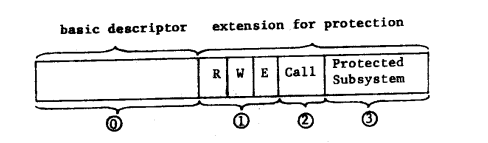
\includegraphics[scale=0.55]{images/descriptor.png}
    \caption{Multics descriptor \cite{protectionSaltzer}}
    \label{fig:descriptor}
\end{figure}

\subsection{Authentication of users}

Whole process of access control lists, access modes, protected subsystems and hierarchical control depends on an 
accurate principal identifier being associated with every process. Accuracy of the identification depends on 
authentication of the user's claimed identity.

Every user is \textit{registered} with \textit{unique name} (convention: last name, plus one or two initials) 
associated with a \textit{password} of up to eight ASCII characters. Also as another measurement, the user may 
(after authenticating) change his password at any time.

When user types a password it is \textit{enciphered} and compared with the stored enciphered version for validity.
All passwords on system are stored in non-invertible cipher (one-way encryption) form, which also acts as additional 
security in case of system dump. 

Plain text passwords are stored \textit{nowhere} on the system. As a result, passwords 
are not routinely know by any system administrator or project administrators.

Additional feature of Multics system password mechanism is that, when user is requested to give his password, the printer 
on his terminal is \textit{turned off}.(Because of endless and penetrable checking of input arguments).


Each login and logout is carefully audited to check for attempts to guess a valid password for a certain user. 
If a user provides incorrect password, the event of an \textit{incorrect login attempt} is noted in \textit{
threat-monitoring log}, and user is permitted to try again, up to ten-times at which point the telephone or network 
connection is broken by the system.

In addition each user is informed of the \textit{date}, \textit{time} and \textit{terminal identification} of last
login to detect past compromises of the users \textit{access rights}, also user is told the number of times his password 
has been given incorrectly since its last correct use in his greeting message. 


\subsection{Primary Memory Protection}

The virtual address space of a Multics process is implemented with an \textit{array of descriptors}, called 
a \textit{descriptor segment}. Every reference to the virtual memory specifies both, segment number (index) and a 
word number within the segment.

The reason why the protection information is associated with the addressing descriptor rather than data itself is, 
in \textit{multiprocessor system} such as Multics, two same processes may be executing at a same time, so single 
protection specification associated with the data is not sufficient.

\begin{enumerate}
    \item Physical address and size of the segment based on this descriptor.
    \item Bits separately controlling permission (read-write-execute).
    \item Control of permission to enter a protected subsystem which has entry points in the segment.
    \item Controls on which protected subsystems may use this descriptor.
\end{enumerate}

Another feature of the descriptors used in Multics is implemented inside the \textit{second} and \textit{third} part of descriptor, 
which can be seen on \textit{Figure} \ref{fig:descriptor}, together they allow hardware enforcement of protected subsystems, 
which are intended to be used only by calls to \textit{designated entry points}, know as \textit{gates}. As a result of this, 
it is possible to construct proprietary programs which cannot be read. They return only statistics rather than raw data.

\textit{Protected subsystems} are formed by using the \textit{third field} of the descriptor extension. Multics force a 
\textit{hierarchical} constraint on all subsystems within a single process. Each subsystem is assigned a number between 
\textbf{0} and \textbf{7}. This scheme is also called \textit{the ring mechanism} or \textit{the rings of protection}. 
The protection rings are defined in the way:
\textit{The higher numbered rings having less privilege than lower numbered rings, and ring 0
containing 'hardcore' supervisor}. Therefore, each subsystem is permitted to use all of those descriptors containing 
protected subsystem numbers greater or equal to its own.

The descriptors are adjusted to provide \textit{only} the amount of access required by the \textit{supervisor} in direct 
harmony of \textit{Design principal number 6}. These mechanism do not prohibit the supervisor from making full use of hardware, 
rather than protection against accidental/exploitation overuse of supervisor privileges.

\subsection{Master Mode}

The convention around protecting \textit{master mode software}, was specified as the master mode procedures
were not to be used outside ring 0. Convention had been defined as of "\textit{each master mode procedure must 
have a master mode pseudo-operation code assembled into location 0}".
The master mode pseudo-operation generates code to test an index register for a value corresponding to an 
entry point in the segment. If the index register is invalid, the master mode pseudo-operation saves the
registers for debugging and shuts the system down.

\subsection{Software Maintenance Procedure}

The system is initialized from a magnetic tape which contains copies of every program residing in the \textit{most protected 
area}. The maintenance of the \textit{Multics software} had been carried out \textbf{online} on a \textit{dial-up 
Multics facility}. A programmer prepared (and debugs) his software for installation, then submits his
software to a \textit{library installer} who copied and recompiled the source code in a \textit{protected 
directory}. 
The software prior installing into the system source and object libraries is checked by library installer.
Ring 0 software is stored on a \textit{system tape} that is reloaded into the system each time it is brought up.
(New system tapes are generated from online copies of the ring 0 software).
The system libraries had been protected against modification by access control list mechanism. In addition 
the library installers had been periodically checked of last modification of all segments in the library to
detect unauthorized modifications.
% Based on:
% setup http://multics-wiki.swenson.org/index.php/Getting_Started
% using http://multics-wiki.swenson.org/index.php/Using_Multics#More_Processing
%
% # --------------------------------------------------------------------------------- #

\section{Running Multics nowadays}

Creating a Multics system or machine nowadays is a bit sketchy process. Since Multics is relying on designated hardware 
such as HIS-645 or 6180 processors (developed by Honeywell) it is not an easy task to do.
You can not simply create \textit{Virtual Machine} from from disk image (ISO). But there are still some options how to do it, 
you can use \textit{simulator/emulator} for such a task. 

MIT in cooperation with BULL runs \href{https://web.mit.edu/multics-history/source/Multics_Internet_Server/Multics_sources.html}{Multics Internet Server} \cite{mitBull}
containing edition of Multics software and documentation, which is useful if you want to try PL/I and rest locally.


\subsection{DPS8-Simulator}

I came across project which still maintain love and desire for running Multics system.
\textbf{RingZero - Multics Reborn} \cite{ringzero} project, created by \textit{Harry Reed} and \textit{Charles Anthony} which is available for 
public \href{http://ringzero.wikidot.com/}{download}. Development takes place on \href{https://gitlab.com/dps8m/dps8m}{GitLab}. 
They provide \textit{DPS8-M simulator}. Still with no much capabilities, but as stated milestone from 11. August 2014:

\begin{displayquote}
\textit{Multics reborn! The dps-8/m SIMH-based simulator booted Multics MR 12.5, came to operator command level, entered 
admin mode, created a small PL/I program, compiled and executed it, and shut down.} \cite{ringzero}
\end{displayquote}

\subsection{How to run Multics on GNU\textbackslash Linux}

Detailed process can be found \href{http://multics-wiki.swenson.org/index.php/Main_Page}{Swenson's Multics Wiki} \cite{setupRingZero}

\begin{enumerate}
    \item \href{http://ringzero.wikidot.com/r2-0-load-and-go}{Download} \textit{Pre-built executable} (so we do not need to build simulator from source).
    \item \href{https://s3.amazonaws.com/eswenson-multics/public/releases/MR12.6f/QuickStart_MR12.6f.zip}{Download} "QuickStar RLV", which provides and already Multics system disk image that is ready to run.
    \item Unzip both archives and put in the same directory in system. Go to directory in terminal and:
\end{enumerate}

\begin{lstlisting}
$> ./dps8 MR12.6f_boot.ini 

DPS8/M emulator (git 2a56f38d)
Production build
#### M_SHARED BUILD ####
System state restored
Please register your system at https://ringzero.wikidot.com/wiki:register
or create the file 'serial.txt' containing the line 'sn: 0'.
FNP telnet server port set to 6180

DPS8/M simulator V4.0-0 Beta        git commit id: c420925a
TAPE: unit is read only
MR12.6f_boot.ini-30> set opcon config=attn_hack=1
Non-existent device
[FNP emulation: listening to 127.0.0.1 6180]
CONSOLE: ALERT
bootload_0: Booting system MR12.6f generated 01/09/17 1119.1 pst Mon.   
1500.2  announce_chwm: 428. pages used of 512. in wired environment.
1500.2  announce_chwm: 706. words used of 1024. in int_unpaged_page_tables.
find_rpv_subsystem: Enter RPV data: M-> [auto-input] rpv a11 ipc 3381 0a

1500.2  load_mst: 946. out of 1048. pages used in disk mst area.
bce (early) 1500.2: M-> [auto-input] bce

Multics Y2K.  System was last shudown/ESD at:
Saturday, April 1, 2017 20:37:12 pst
Current system time is: Sunday, April 19, 2020 7:00:16 pst.
Is this correct? M-> [auto-input] yes

The current time is more than the supplied boot_delta hours beyond the
unmounted time recorded in the RPV label.  Is this correct? M-> [auto-input] yes

The current time I'm using is more than 12 hours
after the last shutdown time recorded in the RPV label.
Are you sure this is correct? M-> [auto-input] yes

bce (boot) 0700.2: M-> [auto-input] boot star

Multics MR12.6f - 04/19/20  0700.4 pst Sun
0700.4  Loading FNP d, >user_dir_dir>SysAdmin>a>mcs.7.6c>site_mcs 7.6c
Received BOOTLOAD command...
0700.4  FNP d loaded successfully


Volumes to be Scavenged:

rpv    (root)
root2  (root)
root3  (root)

Ready
0700  as   as_init_: Multics MR12.6f; Answering Service 17.0
0700  as   LOGIN              IO.SysDaemon dmn cord (create)
0700  as   LOGIN              Backup.SysDaemon dmn bk (create)
0700  as   LOGIN              IO.SysDaemon dmn prta (create)
0700  as   LOGIN              Utility.SysDaemon dmn ut (create)
0700  as   LOGIN              Volume_Dumper.Daemon dmn vinc (create)
0700  as   LOGIN              Scavenger.SysDaemon dmn scav1 (create)
0700  as   as_mcs_mpx_: Load signalled for FNP d.
0700  bk   
0700  cord Enter command:  coordinator, driver, or logout:
-->  cord
0700  bk   r 07:00 0.194 30
0700  bk   
-->  bk
0700  prta Enter command:  coordinator, driver, or logout:
-->  prta
0700  ut   copy_dump: Attempt to re-copy an invalid dump.
0700  ut   delete_old_pdds: Some directory or segment in the pathname is not listed in the VTOC. Unable to salvage >pdd.!BBBKPBBzF
0700  ut   jWCfq. Will attempt to delete it.
0700  ut   delete_old_pdds: Some directory or segment in the pathname is not listed in the VTOC. Unable to salvage >sl1.!BBBKPBBzF
0700  ut   jWCfq. Will attempt to delete it.
0700  vinc 
0700  vinc r 07:00 0.197 25
0700  vinc 
-->  vinc
0700  scav1 Created >system_control_1>scav1.message
0700.5  scavenger: Begin scavenge of dska_00a by Scavenger.SysDaemon.z
0700  scav1 Scavenging volume rpv of logical volume root
0700  as   sc_admin_command_: Utility.SysDaemon.z: delete_old_pdds
0700  ut   send_admin_command: Execution started ... 
0700.7  vtoce_stock_man: Attempt to deposit free vtocx 4037 on dska_00
0700.7  vtoce_stock_man: Attempt to deposit free vtocx 4036 on dska_00
0700  ut   completed.
0700.7  scavenger: Scavenge of dska_00a by Scavenger.SysDaemon.z completed.
0700.7  scavenger: Begin scavenge of dska_00b by Scavenger.SysDaemon.z
0700  scav1 Scavenging volume root2 of logical volume root
0700  ut   monitor_quota: The requested action was not performed. 
0700  ut   The quota of >dumps is 0, a record limit needs to be specified.
0700.7  RCP: Attached tapa_00 for Utility.SysDaemon.z
0700  ut   
0700  ut   Records   Left  %    VTOCEs   Left  %   PB/PD  LV Name
0700  ut   
0700  ut   166172   99180  60   42218   33972  80  pb     root
0700  ut   
0700  ut   r 07:00 0.505 477
0700  ut   
-->  ut
0700.7  RCP: Detached tapa_00 from Utility.SysDaemon.z
0700.7  RCP: Attached rdra for Utility.SysDaemon.z
0700.7  RCP: Detached rdra from Utility.SysDaemon.z
0700.7  RCP: Attached puna for Utility.SysDaemon.z
0700.7  RCP: Detached puna from Utility.SysDaemon.z
0700.7  RCP: Attached prta for Utility.SysDaemon.z
0700.7  RCP: Detached prta from Utility.SysDaemon.z
0700.9  scavenger: Scavenge of dska_00b by Scavenger.SysDaemon.z completed.
0700  scav1 Scavenging volume root3 of logical volume root
0700.9  scavenger: Begin scavenge of dska_00c by Scavenger.SysDaemon.z
0701.1  scavenger: Scavenge of dska_00c by Scavenger.SysDaemon.z completed.
\end{lstlisting}

Your Multics system is up and running. The terminal shell in which you started the simulator and Multics is now the operator console.


The simulator should be listing on TCP port 6180 and if you connect to that port using telnet, you should be able to login. 

\begin{lstlisting}
$> telnet localhost 6180

Trying ::1...
telnet: connect to address ::1: Connection refused
Trying 127.0.0.1...
Connected to localhost.
Escape character is '^]'.
HSLA Port (d.h000,d.h001,d.h002,d.h003,d.h004,d.h005,d.h006,d.h007,d.h008,d.h009,d.h010,d.h011,d.h012,d.h013,d.h014,d.h015,d.h016,d.h017,d.h018,d.h019,d.h020,d.h021,d.h022,d.h023,d.h024,d.h025,d.h026,d.h027,d.h028,d.h029,d.h030,d.h031)? 
Attached to line d.h000

Multics MR12.6f: Installation and location (Channel d.h000)
Load = 5.0 out of 90.0 units: users = 5, 04/19/20  0706.0 pst Sun
\end{lstlisting}

Now you can login as SysAdmin

\begin{lstlisting}
$> login Repair -cpw    # flag to change password

Password:
New Password:
New Password Again:

Your password was given incorrectly at 04/15/20  0706.4 pst Sun from ASCII term
\cinal "none".      
# Audit Trial in use, I've put password once incorrectly

Password changed.
You are protected from preemption.
Repair.SysAdmin logged in 04/19/20  0706.7 pst Sun from ASCII terminal "none".

New messages in message_of_the_day:

Welcome to the Multics System.

print_motd:  Created >user_dir_dir>SysAdmin>Repair>Repair.value.
r 07:06 0.208 31

M->         # you can start using Multics
\end{lstlisting}

With this running Multics you can do:

\begin{itemize}
    \item Logging into an Existing Account
    \item Logging in as an Anonymous User
    \item Creating Directories
    \item Listing the Contents of Directories
    \item Entry Names
    \item Editing files (Emas, qedx, edm, Teco)
    \item Printing files
    \item Setting Time Zone
\end{itemize}

\textbf{Quick overview of these capabilities will be demonstrated during my presentation}.



% Based on:
% Multics Security Evaluation: Vulnerability analysis
% Paul A. Karger (2nd Lt, USAF)
% Roger R. Schell (Major, USAF)



% # --------------------------------------------------------------------------------- #
\section{Multics Security Evaluation by USAF}

Since on running DPS8-M simulator, you can not really breach security controls. I will describe in short well known evaluation of 
Multics system and how they were able to exploit vulnerabilities in system. 

\textbf{The security evaluation is described in \textit{Multics Security Evaluation: Vulnerability analysis} by P.A. Karger and R.R. Schell} \cite{AnalysisKargerSchell}.

Evaluation of the security of the Multics system had been carried out on the \textit{HIS 645} 
Multics Systems installed at the \textit{Massachusetts Institute of Technology} and at the 
\textit{Rome Air Development Center} in span of March 1972 and June 1973.

The main purpose for this evaluation had been the lack of effective \textit{multi-level security controls}
in US military. The term multi-level (from US Military point of view) means, in the most general case, 
those controls needed to process several levels of \textit{classified material}, from unclassified 
through compartmented top secret in a \textit{multi-processing multi-user computer system with simultaneous 
access} to the system by users with different levels of clearances.

The lack of such effective systems in those days has led the \textit{US Military} to operate computers
in closed environment in which system had been dedicated to the highest level of classified material and
all users had been required to be cleared to \textit{that} level.
Such a systems resulted in extreme insufficient manpower utilization and high costs of deployed systems,
mainly becuase of quantity of dedicated systems. 

Requirements of the \textit{Air Force Data Service Center} (AFDSC) were to be providen with 
\textit{responsive interactive time-shared computer services} to users within the Pentagon
at all \textit{classification levels}. From \textit{unclassified} to \textit{top secret} clearance level.
AFDSC in particular did not wish to incur the expense of \textit{multiple computer systems} nor the expense of 
\textit{encryption devices} for remote terminals which would otherwise be processing unclassified materials.

\textbf{Several more analysis has been done in years after, but this analysis was the key 
for Multics to gain B2 security evaluation mark.}


\subsection{State of "current systems" in early 70's}
% Operating systems does not considered the security as fundamental requirement

The internal controls of current computers repeatedly had been shown \textit{Insecure} through many
\textit{penetration exercises} on system such as \textit{WWMCCS GCOS} and \textit{IBM OS/360/370}.
This insecurity of internal controls had been fundamental weakness of \textit{these} operating systems 
and cannot be corrected by \textit{"patches"}, \textit{"fix-ups"} and \textit{"add-ons"} to these systems.
Rather a \textit{fundamental re-implementation} using an integrated hardware and software design which would 
consider \textbf{security as fundamental requirement}.

It is not sufficient to use a team of experts to \textit{test} the security controls of a system. Such a 
\textit{ZARF "tiger team"} can only show the existence of vulnerabilities but \textit{cannot} 
prove their \textit{non-existence}.

\subsection{Reference Monitor}

The concept of \textit{reference monitor} had been introduced by the \textit{ESD Computer Security 
Technology Panel}. This reference monitor is that hardware and software \textit{combination} which 
must monitor \textbf{all} references by \textbf{any program} to \textbf{any data anywhere} in the 
system to ensure that the security rules are followed, which are defined by:
\begin{itemize}
    \item The monitor must be tamper proof.
    % Tamper = to touch or make changes to something that you should not, 
    % usually without enough knowledge of how it works or when you are trying to damage it
    \item The monitor must be invoked for every reference to data anywhere in the system
    \item The monitor must be small enogh to be \textit{proven correct} 
\end{itemize}

Systems such as GCOS and OS/360 meet just first requirement. The second requirement was generally not met by
systems contemporary in \textit{60s} and \textit{70s}, since they usually include \textit{bypasses} to permit
special software top operate.
The most important, operating systems in those days had been so \textit{large}, so \textit{complex} and 
so \textit{monolithic} that one could not begin to attempt a formal proof or certification of their current 
implementation. 

\subsection{Approach Plan}

An attempt was to be made to operate with same type of ground rules under which a real agent would operate.
That is, with each penetration, and attempt would be made to extract or modify sensitive system data 
without detection by the \textit{system maintenance} or \textit{administrative personnel}.
Several exploitation's had been discovered, such as changing access fields in SDW's, changing protected 
identities in the PDS, inserting trap doors into system libraries and accessing the system password file.

In this paper we are not going to to describe all the vulnerabilities shown by this evaluation, rather just those 
interesting and with the most significant impact on contemporary development of operating systems and its 
security's control systems.

% \subsection{Hardware Vulnerabilities}

\subsection{Subverter routine}

To attempt a gross measure of the rate of security sensitive component failure, a procedure called the 
\textit{subverter} was written to sample the security sensitive hardware on frequent basis, testing for 
component failures which could compromise the security controls.
The subverter was run in the background of an interactive process, once each minute. The subverter was run 
over 1100 hours in a year period on the \textit{MIT 645 System}, during these operating hours no security sensitive 
component failures were detected.
Which points at and gave great result about the concert in a system processing multi-level classified material.
If the hardware is prone to error, potential security vulnerabilities become a significant problem.

\subsection{Instruction Access Check Bypass}

While experimenting with the hardware subverter, a sequence of code was observed which would cause the hardware 
of the 645 to \textit{bypass access checking}. Specifically the \textit{execute} instruction in certain cases 
would permit the executed instruction to access a segment for \textit{reading} or \textit{writing} without the 
corresponding permissions in the SDW.
This vulnerability occurred when the execute instruction was in certain restricted locations of a segment with 
at least \textit{read-execute} permission.
The exact layout of instructions and indirect words was crucial, otherwise the \textit{access checks} were done 
properly.
This bug represents a violation of one of the most fundamental rules of the Multics design concept - the checking 
of \textbf{every} reference to a segment by the hardware.

% \subsection{Software Vulnerabilities}

\subsection{Insufficint Argument Validation}

On the 645 CPU rings mechanism have not been implemented in the way of hardware. (Only after several years on HIS 6180 CPU.) 
Therefore, the protection rings had been implemented by providing \textit{eight descriptor segments} for each user, one 
descriptor segment per ring.
Because the 645 Multics system must simulate \textit{protection rings} in software, there is no direct hardware 
validation of arguments passed in a subroutine call from a \textit{less privileged ring} to \textit{more 
privileged ring}. Some form of validation is required, because a malicious user could call a ring 0 routine 
that stores information through a user supplied pointer.
If the malicious user supplied a pointer to data to which ring 0 had \textit{write} permission but to which the 
user ring did not, ring 0 could be \textit{"tricked"} into causing a security violation.

To provide validation, the 645 \textit{software ring crossing mechanism} requires all gate segments to declare to 
the \textit{"gatekeeper"} the following information:
\begin{enumerate}
    \item number of arguments expected
    \item data type of each arguments
    \item access requirements for each argument - read only or read/write
\end{enumerate} 
This information is stored by convention in specified locations within the \textit{gate segment}. The gatekeeper 
invokes an argument validation routine that inspects the argument list being passed to the gate to ensure that the 
declared requirements are met. If any test fails, the argument validator aborts the call and signals the \textit{"
gate\textunderscore error"} in the calling ring.

In 1973, a vulnerability was identified in the argument validator that would permit the \textit{"fooling"} of ring 0 
programs.
The argument validator's algorithm to validate read or read/write permission was as this:
\begin{enumerate}
    \item Copy the argument list into ring 0 to prevent modification of the argument list by a process 
    running on another CPU in the system while the first process is in ring 0 and has completed argument validation
    \item Force indirection through each argument pointer to obtain the segment number of the target argument
    \item Look up the segment in the calling ring's descriptor segment to check for read or write permission
\end{enumerate}

The vulnerability is as follows:
\begin{itemize}
    \item An argument pointer supplied by the user is constructed to contain an IDC modfier that causes the first 
    reference through the indirect chain to address a valid argument.
    \item The first reference is the one made by the argument validator.
    \item The reference through the IDC modifier increments the address field of the tally word causing it to point 
    to a different ITS pointer which points to an argument which is writable in ring 0 \textbf{only}.
    \item The second reference through this modifier indirect chain is made by the ring 0 program which proceeds 
    to \textbf{write data where it should not}. 
\end{itemize}
%# TODO add 'Figure 5. Insufficient Argument Validation' .pdf (p) 28

This vulnerability resulted from violation of a basic rule of the Multics design, that \textit{all arguments to a more 
privileged ring must be validated}.
The problem was no in the fundamental design, but the lack of \textit{ring hardware} on HIS-645 CPU system.

\subsection{Master Mode Transfer}

The HIS-645 CPU has a \textit{master mode} in which privileged instructions may be executed and in 
which \textit{access checking is inhibited} although address translation through segment and page 
tables is retained. 
The original design of Multics protection rings called for master mode code to be restricted to ring 0 by convention.
This convention caused the \textit{fault handling mechanism} to be excessively expensive due to necessity of switching
from user ring into ring 0 and out again using the full software ring crossing mechanism.

Therefore it was proposed and implemented that the \textit{signaller} module  was permitted to run in the user 
ring to speed up fault processing.

The analysis shows that master mode procedures in the user ring represents a fundamental violation of the Multics 
security concept. Violating this concept moves the security controls from the basic hardware and software mechanism 
to the cleverness of the systems programmer who, \textit{being human, makes mistakes and commits oversights}
The master mode procedures become classical "supervisor calls" with no rules for sufficient security checks.

The master mode \textit{pseudo-operation} code was designed only to protect master mode procedures from random calls 
within ring 0. It was not designed to withstand the attack of a malicious user. By moving the signaller into the user 
ring, the designers allowed a user leaving a core dump and therefore to crash the system.


\subsection{Dump and Patch Utilities}

\textit{This section shows the exploitation by a remote user online}.

To provide support to the system maintenance personnel, the Multics system includes commands to \textit{dump} or 
\textit{patch} any word in the \textbf{entire virtual memory}. These utilities are used to make online repairs while 
the system continues to run. These commands are dangerous, because they \textit{bypass} all security controls to 
access otherwise protected information, and if misused, it can cause crash of the entire system.

To protect the system, these commands are implemented by special privileged \textit{gates} into ring 0. The access control 
lists on these gates restrict their use to system maintenance personnel by name and authenticated by the login procedure.

Dump and patch utilities would be of a great use to a system penetrator, because they can be used to "do his job". These 
utilities are prevented from misuse by \textit{ACL} and \textit{audit trial}, but using  \textit{insufficient argument
validation}, \textit{master mode transfer} and \textit{unlocked stack base} vulnerabilities, these procedural controls 
may be bypassed and the penetrator can implement his own dump and patch utilities. Can be seen on \textit{Figure \ref{dump/patch}}.

\begin{figure}
    \centering
    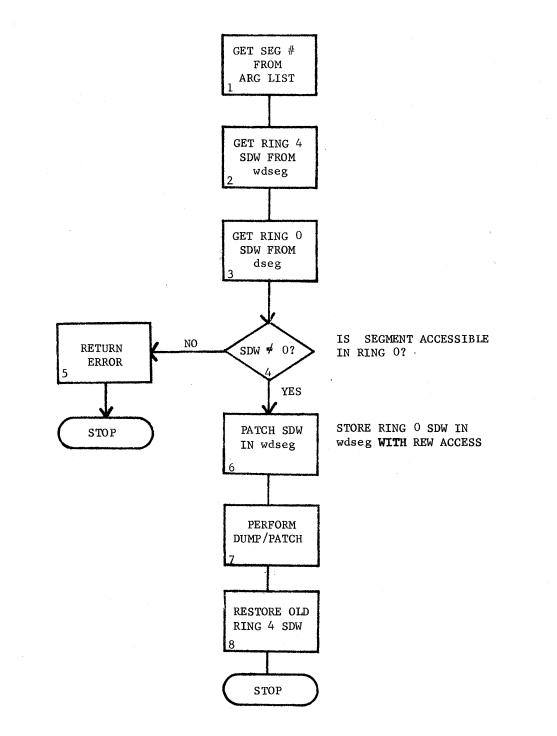
\includegraphics[scale=0.4]{images/dumpPatch.png}
    \caption{Dump/patch utility using insufficient argument validation}
    \label{dump/patch}
\end{figure}

\subsection{Violating The User Identification}

In the need for a protected identification of every user, his ID must be compared with access control list entries 
to determine whether a user may access some segment as stated in Security Controls section.
This identification is established when the user logs into Multics and is authenticated by the password.

The user identification in Multics is stored in a per-process segment called the \textit{process data segment} (PDS).
PDS resides in ring 0 and contains many constants used in ring 0 and the ring 0 procedure stack. The PDS must be 
accessible to any ring 0 procedure within a user's process and must be accessible to ring 4 master master mode 
procedures such as signaller.

Therefore as stated above section about Dump and Patch utilities vulnerability, these can dump and patch portions of the 
PDS, thus \textit{forging the non-forgeable user identification}.
This capability provides the penetrator with an ultimate exploitation weapon. The penetrator can undetechably act as any 
user of the system, including the \textit{system administrator} or \textit{security officer}, immediately assuming that 
user's access privileges.

\subsection{Value of the Password File}

The password file is often kept enciphered. A great deal of effort may be required to invert such a cipher, if the cipher 
is even invertible at all.
The password file is generally the most protected file in a computer system. If the penetrator has succeeded in breaking 
down internal controls to access the password file, he can also \textbf{access every other file in the system}.
The login path to a system is generally the most carefully audited to attempt to catch \textit{unauthorized} password use.
The penetrator risks \textit{detection} if he uses an unauthorized password.

So in this point we can assume that accessing the system password file is of minimal value to a penetrator for reasons 
stated above.

\subsection{Modifying Audit Trials}

Audit trails are frequently put into computer systems for the purpose of detecting breaches  of  security. 
For example, a record of last login time printed when a user logged in could detect the unauthorized 
use of a user’s password and identification.
Sometimes it is not convenient for the penetrator to bypass an audit, if the audit trial is kept online, 
it may be easier to allow the audit to take place and then go back and modify the evidence of wrong doing.
Every segment in Multics carries with it audit information on the \textit{Date Time last Used} (DTU) and
\textit{Date Time last Modified} (DTM). These dates are maintained by an \textit{audit mechanism} at a low 
level in the system.

A routine called "set\textunderscore dates" is provided among the various subroutine calls into ring 0, which is used when 
a segment is retrieved from a \textit{backup tape} to set the segments DTU and DTM to the values at the time the 
segment was backed up. This routine is supposed to be callable only by system maintenance personnel (ring 0).
However, since the penetrator can change his user identification, this restriction proves to be no barrier.

To access a segment penetrator simply:
\begin{enumerate}
    \item Change user ID to access segment.
    \item Remember old DTU and DTM.
    \item Use or modify the segment.
    \item Change user ID to system maintenance.
    \item --do whatever you want--
    \item Reset DTU and DTM to old values.
    \item Change user ID back to old value.
\end{enumerate}


\subsection{Trap Door Insertion}

In short, trap door is a a feature or defect of a computer system which allows surreptitious unauthorized 
access to data and system itself. When trap door is inserted, it must be well hidden to avoid detection by system
maintenance personnel.
Trap doors can be inserted in many places:
\begin{itemize}
    \item At the facility which the system is produced.
    \item During the distribution phase. If updates are sent via insecure communications.
    \item During the installation and operation of the system at user's site.
\end{itemize}

Trap doors can be easily hidden in changes to the binary code of compiled routine. Such a change can be 
detected only by comparing bit by bit the object code and the compiler listing. Which can be easily secured 
by regularly recompile of all modules of the system to eliminate such a trap doors.
However, if the compiler trap door is inserted to permit object code trap doors to survive even a complete 
recompilation of entire system. 
In Multics most of the ring 0 supervisor is written in PL/I. Penetrator could insert trap door in the PL/I and 
easily delist the desired code to be recompiled.
Since the PL/I compiler is itself written in PL/I, the trap door can \textit{maintain itself, even if the 
compiler is recompiled}.

The actual insertion of the trap door was done by following steps:
\begin{enumerate}
    \item Change user ID to project SysLib.
    \item Make patch in the object archive copy of "check\$device\underline{} name" in >ldd>hard>object.
    \item Reset DTM on object archive.
    \item Mark patch in bound archive copy of "check\$device\underline{} name" in >ldd>hard>bound\underline{}components.
    \item Reset DTM on bound archive.
    \item Reset user ID back to old value.
\end{enumerate}

\subsection{Conclusion by Schell and Karger}

The primary conclusion one can reach from this analysis is that Multics is \textit{not currently a secure system} (1973).
But on the other hand, it is \textbf{significantly more secure} than any other system.



\section{Significance and Influence of Multics}

As we could read in previous sections, it is clear that Multics was the first system, which considered \textit{security} a 
\textbf{necessity}, not an additional feature. Multics was designed to be secure from the beginning. This fact is in modern 
operating systems taken for granted. In the 1985 the system was awarded the B2 security rating by the NCSC, the first 
(and for years only) system to get a B2 rating.

Multics was written in the \textit{PL/I} language (created by IBM in 1964), only part of the operating system was implemented 
in \textit{assembly} language. Writing operating system in a \textit{high-level} (not in today's standards) language was a 
radical idea at the time. In addition to PL/I, Multics supports BCPL, BASIC, FORTRAN, LISP, COBOL, ALGOL68 and additionally C and Pascal. 

Multics provided \textit{first commercial relational database} product. The \textit{MRDS}, Multics Relational Data Store.\cite{mindpride}

All systems in early 70's was designed to be able to run 24/7, but only Multics had capability to add or remove CPUs, memory, 
I/O controllers and disk drives from system configuration while the system is running.

The most notable influence on other operating system, which we can still see today is in GNU/Linux based systems.
Part of it is because inventors of \textbf{UNIX} \textit{Ken Thompson} and \textit{Dennis Ritchie} (also inventor of C language), 
worked on Multics until \textit{Bell Labs} dropped out of the Multics development in 1969.

Ken Thompson was "inspired" by \textit{access control list mechanism}, which was implemented in UNIX and was also one of the
primary security measurements in the system.

The idea of having the \textit{command processing shell} to be an ordinary slave program came from the Multics design, 
and a predecessor program on \textit{CTSS} by \textit{Louis Pouzin} called \textbf{RUNCOM}.\cite{multicians}

The value of Multics in UNIX early development ideas could be also seen at the \textit{50th Anniversary} of the Unix creation.
One of the articles, by \textit{Richard Jensen} is called \textit{Unix at 50: How the OS that powered smartphones started from 
failure}, which direct reference to Multics. Such articles often say: 
\begin{displayquote}
"Multics failed. The Bell Labs computer guys then invented their own system, Unix, and Unix succeeded.
\end{displayquote}
On the other hand, Multics did not fail, it accomplished almost all of its stated goals. Unix succeeded too, solving a different problem.
\newline \newline
Next time, when you "ssh-into" your remote server and see greeting such as this:
\begin{lstlisting}
    Last login: Fri Apr 17 13:52:12 2020 from 88.212.40.17}
\end{lstlisting}
You can think of \textbf{Multiplexed Information and Computing Service}.


\begin{displayquote}
\textit{
"To what extent should one trust a statement that a program is free of Trojan horses? 
Perhaps it is more important to trust the people who wrote the software."
}
\textbf{Ken Thompson} \cite{thompson}
\end{displayquote}

\section{Glossary}
\begin{itemize}
    \item CTSS - The Compatible Time-Sharing System, \href{https://www.youtube.com/watch?v=Q07PhW5sCEk}{IBM 7090 and young prof. Corbato about Timesharing on WGBH-TV (1963)}
    \item Descriptor - Contents of an SDW.
    \item Gate - Segment that allows transfer of control between rings in a controlled fashion. Each gate segment has a vector of entries at its start.
    \item IBM OS\textbackslash 360\textbackslash 370 - Family of mainframe computer system developed by IBM.
    \item IDC - Incerement address, Decrement tally, and Continue
    \item PDS - Process Data Segment
    \item PL\textbackslash I - Programming Language \#1, invented by George Radin of IBM in 1964
    \item RCU - Restore Control Unit (ring 0 instruction)
    \item Signaller - Module responsible for processing faults (master mode procedure)
    \item SDW - Segment Descriptor Word. An element of a process's descriptor segment; the hardware-accessible data element that defines a segment and the process's access rights to it.
    \item Subverter - Program written by the Project ZARF team.
    \item WWMCCS GCOS -  The Worldwide Military Command and Control System General Comprehensive Operating Supervisor
    \item ZARF - Code name for Air Force/MITRE tiger team project that cracked Multics security in 1973.
\end{itemize}





\bibliographystyle{ACM-Reference-Format}
\bibliography{library}


\end{document}
